%
\chapter{RTC : Réseau Téléphonique Commuté}
%
%
    \section{Analyse sur un lien}
        \label{seullien} % label pour reference
%
        \subsection{Énoncé}
%
            \paragraph{}
Considérons un lien d'un réseau à commutation de circuits permettant de véhiculer de la voix téléphonique.
%
            \begin{figure}[h]
                \centering
                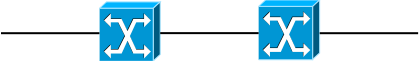
\includegraphics[scale=0.7]{RSC/1-1.png}
                \caption{ Schéma du réseau à commutation de circuit étudié }
                \label{ Schema du reseau a commutation de circuit }
            \end{figure}
%
            \paragraph{}
Chacune des connexions nécessite un débit de $64 \ \text{Kb}.\text{s}^{-1}$ de façon bi-directionnel.
On peut multiplexer simultanément $C$ appels téléphoniques sur ce lien.
%
            \paragraph{}
Le nombre d'utilisateurs est suffisamment grand pour supposer que les arrivées des nouveaux appels suivent une loi de paramètre $\lambda$, les durées des appels sont supposées suivre une loi exponentielle de paramètre $\mu$ avec ($\frac{1}{\mu} = 3 \ \text{minutes}$).
%
%
\clearpage
%
%
        \subsection{Probabilité de blocage d'appel en fonction de la charge $\rho$ et de la capacité $C$}
%
            \[ P(\text{blocage}) = \frac{ \frac{ \rho^C }{ C! } }{ \sum\limits_{i=0}^C \frac{ \rho^i }{ i! } } \]
%
            \begin{center}
                avec $\rho$ la charge et $C$ la capacité.
            \end{center}
%
            \paragraph{}
Voici les résultats de ce calcul, obtenus par notre script Python inclus en annexe \ref{seullien-script}
            \begin{figure}[h]
                \centering
                \begin{gnuplot}[terminal=epslatex, terminaloptions=color dashed]
                    set xlabel 'Capacité'
                    set ylabel 'Taux de rejet'
                    plot "qnap/partie1/calcul.p1.q1.data" u 1:( $2 ==10 ? $3 : 1/0) w l t "Charge de 10", \
                            "qnap/partie1/calcul.p1.q1.data" u 1:( $2 ==20 ? $3 : 1/0) w l t "Charge de 20", \
                            "qnap/partie1/calcul.p1.q1.data" u 1:( $2 ==30 ? $3 : 1/0) w l t "Charge de 30", \
                            "qnap/partie1/calcul.p1.q1.data" u 1:( $2 ==40 ? $3 : 1/0) w l t "Charge de 40", \
                            "qnap/partie1/calcul.p1.q1.data" u 1:( $2 ==50 ? $3 : 1/0) w l t "Charge de 50", \
                            "qnap/partie1/calcul.p1.q1.data" u 1:( $2 ==50 ? $3 : 1/0) w l t "Charge de 50", \
                            "qnap/partie1/calcul.p1.q1.data" u 1:( $2 ==60 ? $3 : 1/0) w l t "Charge de 60", \
                            "qnap/partie1/calcul.p1.q1.data" u 1:( $2 ==70 ? $3 : 1/0) w l t "Charge de 70", \
                            "qnap/partie1/calcul.p1.q1.data" u 1:( $2 ==80 ? $3 : 1/0) w l t "Charge de 80"
                \end{gnuplot}
                \caption{Graphique des résultats de l'étude théorique.}
                \label{pic:p1q1}
            \end{figure}
%
%
\clearpage
%
%
        \subsection{Simulation de cette probabilité de blocage}
%
            \paragraph{}
Pour une charge $10 < \rho < 70$ et pour une capacité $\rho < C < 2*\rho$, on obtient les resultats suivants.
        \begin{figure}[h]
            \centering
            \begin{gnuplot}[terminal=epslatex, terminaloptions=color dashed]
                set xlabel 'Capacité'
                set ylabel 'Taux de rejet'
                plot "qnap/partie1/p1.q2.data" u 2:( $1 ==10 ? $5 : 1/0) w l t "Charge de 10", \
                        "qnap/partie1/p1.q2.data" u 2:( $1 ==20 ? $5 : 1/0) w l t "Charge de 20", \
                        "qnap/partie1/p1.q2.data" u 2:( $1 ==30 ? $5 : 1/0) w l t "Charge de 30", \
                        "qnap/partie1/p1.q2.data" u 2:( $1 ==40 ? $5 : 1/0) w l t "Charge de 40", \
                        "qnap/partie1/p1.q2.data" u 2:( $1 ==50 ? $5 : 1/0) w l t "Charge de 50", \
                        "qnap/partie1/p1.q2.data" u 2:( $1 ==50 ? $5 : 1/0) w l t "Charge de 50", \
                        "qnap/partie1/p1.q2.data" u 2:( $1 ==60 ? $5 : 1/0) w l t "Charge de 60", \
                        "qnap/partie1/p1.q2.data" u 2:( $1 ==70 ? $5 : 1/0) w l t "Charge de 70", \
                        "qnap/partie1/p1.q2.data" u 2:( $1 ==80 ? $5 : 1/0) w l t "Charge de 80"
            \end{gnuplot}
            \caption{Graphique des résultats de la simulation.}
            \label{pic:p1q2}
        \end{figure}
%
%
%
        \subsection{Comparaison des taux de blocage expérimentaux et théoriques}
            \paragraph{}
On constate que les resultats sont similaires, les erreurs de simulation sont gommées par le nombre de simulations important (cela réduit les écarts aléatoires) et leur longue durée (ce qui assure un régime stable).
%
%
    \clearpage
%
%
%
    \section{Analyse sur un réseau de trois commutateurs}
%
        \subsection{Énoncé}
%
            \paragraph{}
Désormais, nous considérons le réseau composé de 3 noeuds.
%
            \begin{figure}[h]
                \centering
                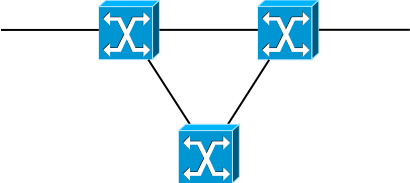
\includegraphics[scale=0.6]{RSC/1-2.png}
                \caption{ Schéma du réseau à 3 commutateurs de circuit étudié }
                \label{ Schema du reseau a 3 commutateurs de circuit }
            \end{figure}
%
            \paragraph{}
Les arrivées sont supposées Poissonniennes sur chacun des nœuds et le trafic se répartit équiprobablement entre les différents nœuds.
Les durées des appels sont supposées exponentielles de même paramètre que dans la première partie (1-a).
Nous ne considérons pas les appels locaux ni les appels qui n'aboutissent pas (absence).
%
%
    \clearpage
%
%
        \subsection{Probabilités de blocage avec le chemin de débordement en cas de saturation du chemin direct}
%
            \paragraph{}
Chaque routeur est représenté par une source qui émet alternativement sur ces deux liens à destination des deux autres routeurs. Lorsqu'un lien est surchargé, un routeur tente d'utiliser le chemin de débordement qu'il a à disposition.
On imagine déjà qu'en cas de forte charge un problème de saturation du système sera inévitable.
%
        \subsection{Comparaison des résultats avec la partie \ref{seullien}}
La simulation se termine brutalement avant d'atteindre une charge de 40, le réseau sature totalement.
Toutefois il est parfois, sur un coup de chance pendant la simulation, possible de s'en rapprocher mais le simulateur n'arrive pas à terminer la simulation par manque de mémoire (limitation de ce vieux programme sûrement compilé en 16 bits).
        \begin{figure}[h]
            \centering
            \begin{gnuplot}[terminal=epslatex, terminaloptions=color dashed]
                set xlabel 'Capacité'
                set ylabel 'Taux de rejet'
                plot "qnap/partie1/p1.q3-2.data" u 2:( $1 ==10 ? $5 : 1/0) w l t "Charge de 10", \
                        "qnap/partie1/p1.q3-2.data" u 2:( $1 ==20 ? $5 : 1/0) w l t "Charge de 20", \
                        "qnap/partie1/p1.q3-2.data" u 2:( $1 ==30 ? $5 : 1/0) w l t "Charge de 30"
            \end{gnuplot}
            \caption{Graphique des résultats de la simulation.}
            \label{pic:p1q3}
        \end{figure}
%
%
    \clearpage
%
%
        \subsection{Problèmes à très forte charge !}
%
            \paragraph{}
Une solution consiste à n'utiliser le chemin de débordement que lorsque celui-ci n'est pas très encombré, c'est à dire en dessous d'un certain seuil d'occupation sur chacun des liens.
Cela revient donc à laisser une marge M aux appels directs.
%
%
            \subsubsection{Commentaires}
%
                \paragraph{}
On imagine que cela évite de bloquer les stations en débordant sur elles puisqu'elle auront chacune une marge de sécurité pour transmettre les appels directs.
%
%
            \subsubsection{Simulation en prenant une marge comprise entre 1 et 3}
%
                \paragraph{}
Plus on augmente la marge, moins l'effet d'auto-saturation provoqué par les débordements est présent, cependant il est normal de constater une légère augmentation du taux de rejet : la marge n'est pas toujours totalement utiliser (l'augmenter ne fera qu'accroître ce phénomène).
        \begin{figure}[h]
            \centering
            \begin{gnuplot}[terminal=epslatex, terminaloptions=color dashed]
                set xlabel 'Capacité'
                set ylabel 'Taux de rejet'
                plot "qnap/partie1/p1.q4.data" u 3:( $1 ==1 ? ($2 == 10 ? $6 :1/0) : 1/0) w l t "Charge de 10", \
                        "qnap/partie1/p1.q4.data" u 3:( $1 ==1 ? ($2 == 20 ? $6 :1/0) : 1/0) w l t "Charge de 20", \
                        "qnap/partie1/p1.q4.data" u 3:( $1 ==1 ? ($2 == 30 ? $6 :1/0) : 1/0) w l t "Charge de 30", \
                        "qnap/partie1/p1.q4.data" u 3:( $1 ==1 ? ($2 == 40 ? $6 :1/0) : 1/0) w l t "Charge de 40"
            \end{gnuplot}
            \caption{Résultats de la simulation pour une Marge de 1.}
            \label{pic:p1q4-m1}
        \end{figure}
        \begin{figure}[h]
            \centering
            \begin{gnuplot}[terminal=epslatex, terminaloptions=color dashed]
                set xlabel 'Capacité'
                set ylabel 'Taux de rejet'
                plot "qnap/partie1/p1.q4.data" u 3:( $1 ==2 ? ($2 == 10 ? $6 :1/0) : 1/0) w l t "Charge de 10", \
                        "qnap/partie1/p1.q4.data" u 3:( $1 ==2 ? ($2 == 20 ? $6 :1/0) : 1/0) w l t "Charge de 20", \
                        "qnap/partie1/p1.q4.data" u 3:( $1 ==2 ? ($2 == 30 ? $6 :1/0) : 1/0) w l t "Charge de 30", \
                        "qnap/partie1/p1.q4.data" u 3:( $1 ==2 ? ($2 == 40 ? $6 :1/0) : 1/0) w l t "Charge de 40"
            \end{gnuplot}
            \caption{Résultats de la simulation pour une Marge de 2.}
            \label{pic:p1q4-m2}
        \end{figure}
        \begin{figure}[h]
            \centering
            \begin{gnuplot}[terminal=epslatex, terminaloptions=color dashed]
                set xlabel 'Capacité'
                set ylabel 'Taux de rejet'
                plot "qnap/partie1/p1.q4.data" u 3:( $1 ==3 ? ($2 == 10 ? $6 :1/0) : 1/0) w l t "Charge de 10", \
                        "qnap/partie1/p1.q4.data" u 3:( $1 ==3 ? ($2 == 20 ? $6 :1/0) : 1/0) w l t "Charge de 20", \
                        "qnap/partie1/p1.q4.data" u 3:( $1 ==3 ? ($2 == 30 ? $6 :1/0) : 1/0) w l t "Charge de 30", \
                        "qnap/partie1/p1.q4.data" u 3:( $1 ==3 ? ($2 == 40 ? $6 :1/0) : 1/0) w l t "Charge de 40"
            \end{gnuplot}
            \caption{Résultats de la simulation pour une Marge de 3.}
            \label{pic:p1q4-m3}
        \end{figure}
%
%
    \clearpage
%
